The temperatures in silicon detector systems are critically important to the performance of these systems. The leakage current shows a pronounced temperature dependence 
\begin{equation}
I\propto T_\text{S}^2e^{-T_\text{A}/T_\text{S}}
\label{eq:leakage_current_temp_dependence}
\end{equation}
where $T_\text{S}$ is the sensor temperature and $T_\text{A}\simeq7000$~K. Leakage currents can become particularly significant after irradiation of the silicon material. The heat generated by these leakage currents in the silicon sensor, together with the heat from front-end electronic components on the detector, needs to be removed by cooling systems. Due to the strong growth of leakage power with temperature there is a critical temperature $T_\text{Crit}$ above which the heat cannot be removed quickly enough, and the detector becomes thermally unstable (`thermal runaway'). The capability of the cooling system to remove this heat is limited by the temperature of the local cold sink (typically the coolant temperature) and the thermal impedance of the heat path between the source (electronics and sensor) and the sink.

In addition, there can be aspects of the front-end electronics that are temperature-dependent. For example, in the strip system for the ATLAS Phase-II upgrade \cite{Collaboration:2017mtb} there are two additional temperature-dependent heat sources. The first is a radiation damage effect in the digital part of the readout electronics (the ABC130 and HCC chips), which is manufactured in 130~nm technology by the CMOS 8RF process (ref). This effect leads to an increase of the digital power in the chip depending on the received dose rate (TID) and the temperature of the chip (ref). This has been first observed in the ATLAS IBL \cite{ATL-INDET-PUB-2017-001}. The other temperature dependence of the power generated by the front-end electronics stems from the converter chip (FEAST (ref)) used in the on-detector DC-DC converter system supplying power to the front-end electronics. 

Even before the limit of thermal stability is reached, knowledge of temperatures in silicon detector systems is important, as they define system parameters like power supply capacity and cable dimensions.

In principle the temperatures in the system for a given set of operational parameters (power density, thermal conductivities, etc.) can be predicted by FEA to an accuracy that is limited only by the quality of the input parameters. However, this is a time-consuming process and can be prohibitively difficult if a number of local heat sources depend non-linearly on the temperature. A simplification to this problem that allows for an analytical solution in the case of a simple heat source topology has been developed in~\cite{Beck:2010zzd}. Here we develop this method further to include several temperature-dependent non-linear heat sources in the front-end electronics. The resulting set of equations cannot be solved analytically anymore, but with little effort using numerical problem solvers. This enables us to predict with some confidence the temperatures and power requirements in the ATLAS strip system throughout Phase-II operation. The results from this prediction have been used throughout the project to consistently dimension the different systems (cooling, power, services, etc.) also with some robustness due to the inclusion of a common set of safety factors. This method can be easily adapted to any other system by adjusting to the system-specific geometries and parameters.

\subsection{The ATLAS strip system}
The strip system for the ATLAS Phase-II upgrade \cite{Collaboration:2017mtb} consists of two parts: the barrel system comprised of four concentric cylindrical barrels, and the two endcaps, which consist of six disks each.

In the barrel, the detector modules are made of square sensors ($96.85\times 96.72$~mm$^2$) with a hybrid on top, which hosts the front-end chips (ABC* and HCC*), but also circuitry to convert the supply voltage of larger than 10~V to the chip voltage of 1.5~V. This circuitry is controlled by the FEAST chip. The modules are glued onto both sides of a composite sandwich that contains two parallel thin-wall titanium cooling pipes embedded in carbon foam (Allcomp K9 - ref)  between two facesheets of UHM carbon fibre (3 layers of K13C2U/EX1515) with a co-cured Kapton/copper low-mass tape. A model of this geometry is shown in Fig.~\ref{fig:barrelgeometry}. During final operation, cooling will be achieved by evaporating CO$_2$ in the cooling pipes with a final target temperature no higher than $-35^\circ$C anywhere on the stave. The geometry of the stave is uniform along its length, with the exception of the end region of the stave, where an End-Of-Structure (EOS) card is mounted on each side, and where the thermal path is degraded by the presence of electrically-insulating ceramic pipe sections. 

\begin{figure}[ht]
\centering
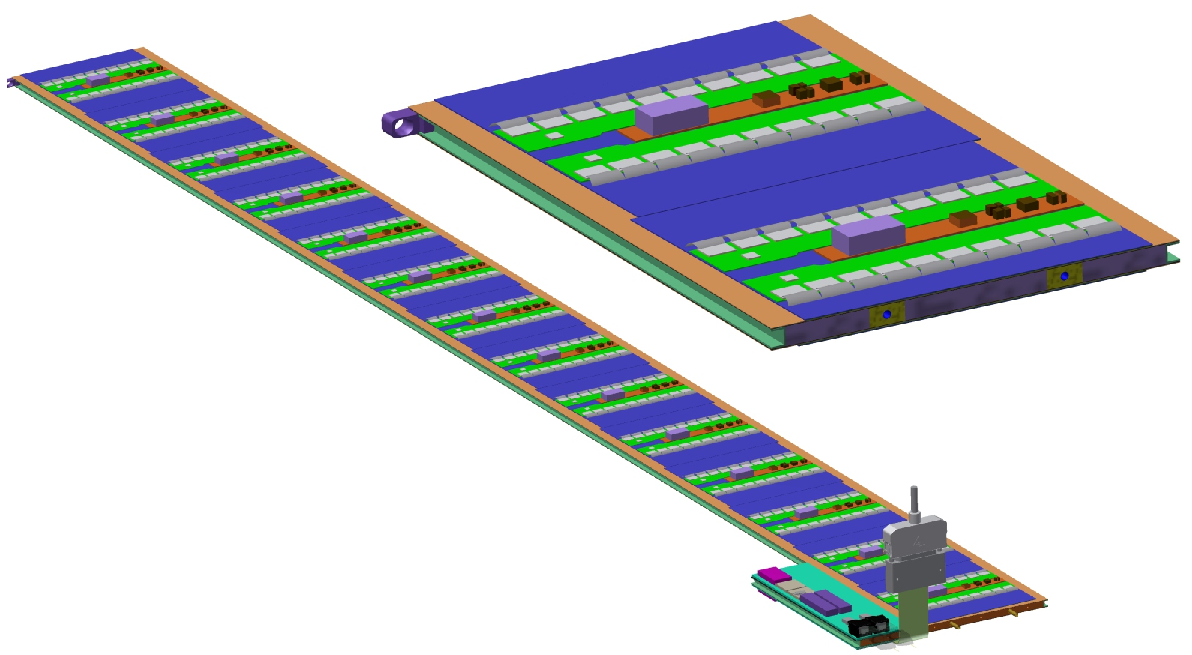
\includegraphics[width=0.8\linewidth]{figures/stave.pdf}
\caption{Strip barrel local support geometry. On the left, a complete stave is shown (note the end-of-structure card in the foreground). The right picture shows a detailed cross-section through the stave with the two cooling pipes visible inside the core. }
\label{fig:barrelgeometry}
\end{figure}

The endcap detector consists of six disks, each containing 32 ``petals'' loaded on
both sides with six silicon modules (twelve in total).
The endcap detector modules consist of six distinct designs located at increasing radius from the
beam pipe and labeled R0 through R5 (where ``R'' stands for ring). Each endcap module consists of one
or two irregularly-shaped silicon sensors, and a varying number of front-end chips on each module
(between 12 and 28 ABCs, and 2 to 4 HCCs). The EOS card is located adjacent to the R5 module, but the
cooling pipes (and not the electrical breaks) run directly underneath it, in contrast to the barrel EOS.
The remaining module and petal core design details are largely identical to the barrel module description above.
Fig.~\ref{fig:endcapgeometry} depicts the geometry of the endcap petal.

\begin{figure}[ht]
\centering
%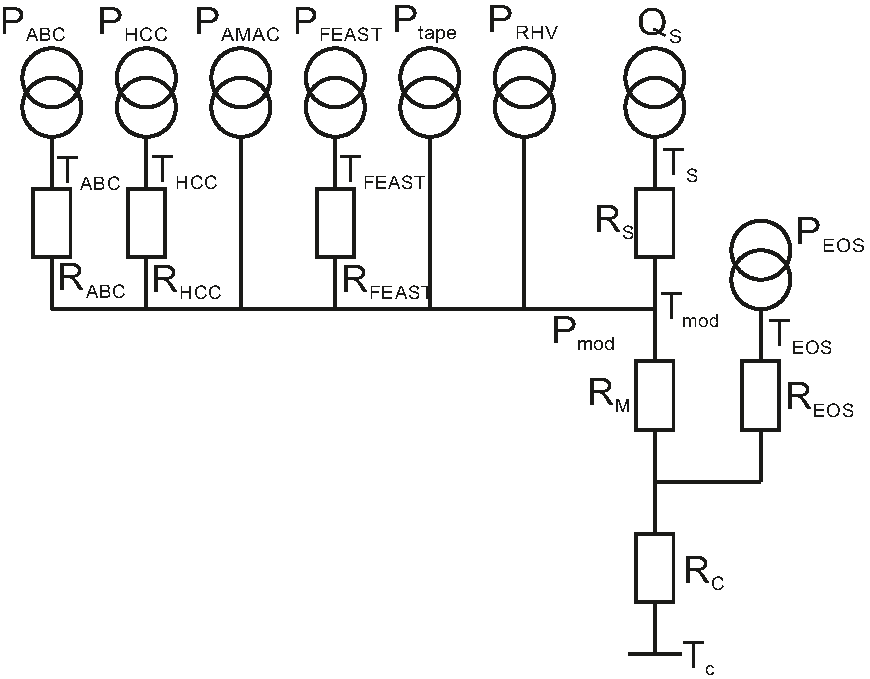
\includegraphics[width=0.6\linewidth]{figures/Thermalmodel.pdf}
\caption{Endcap strip geometry}
\label{fig:endcapgeometry}
\end{figure}

\subsection{Radiation environment}
A key input to the calculation is the radiation environment of the strip system, as several inputs depend on radiation damage effects. The sensor leakage current is a function of the fluence expressed in 1~MeV neutron-equivalents, and the TID effect on the digital chip current will be parametrized as a function of the total ionizing dose rate (more details on its dependencies can be found in Section~\ref{fig:feast_eff}). 

As can be seen in Fig.~\ref{fig:radiation}, both of these quantities display a weak dependence on $z$ in the barrel, whereas they vary significantly along $r$ and $z$ over the length of the endcap petals. Because of this, and the linear uniformity of the stave compared to the more complex geometry along a petal, we modelled only two types of modules for the barrel (a generic module along the linear part of the stave and the module next to the end-of-structure card), but six different types of modules in a petal.
% Note here: the fluence is a justification for modeling layer 0-3 separately, and using
% the flux/TID to model 6 separate versions of a petal.
% The module design justifies 2 (6) different module types in the barrel (endcap).

\begin{figure}[ht]
\centering
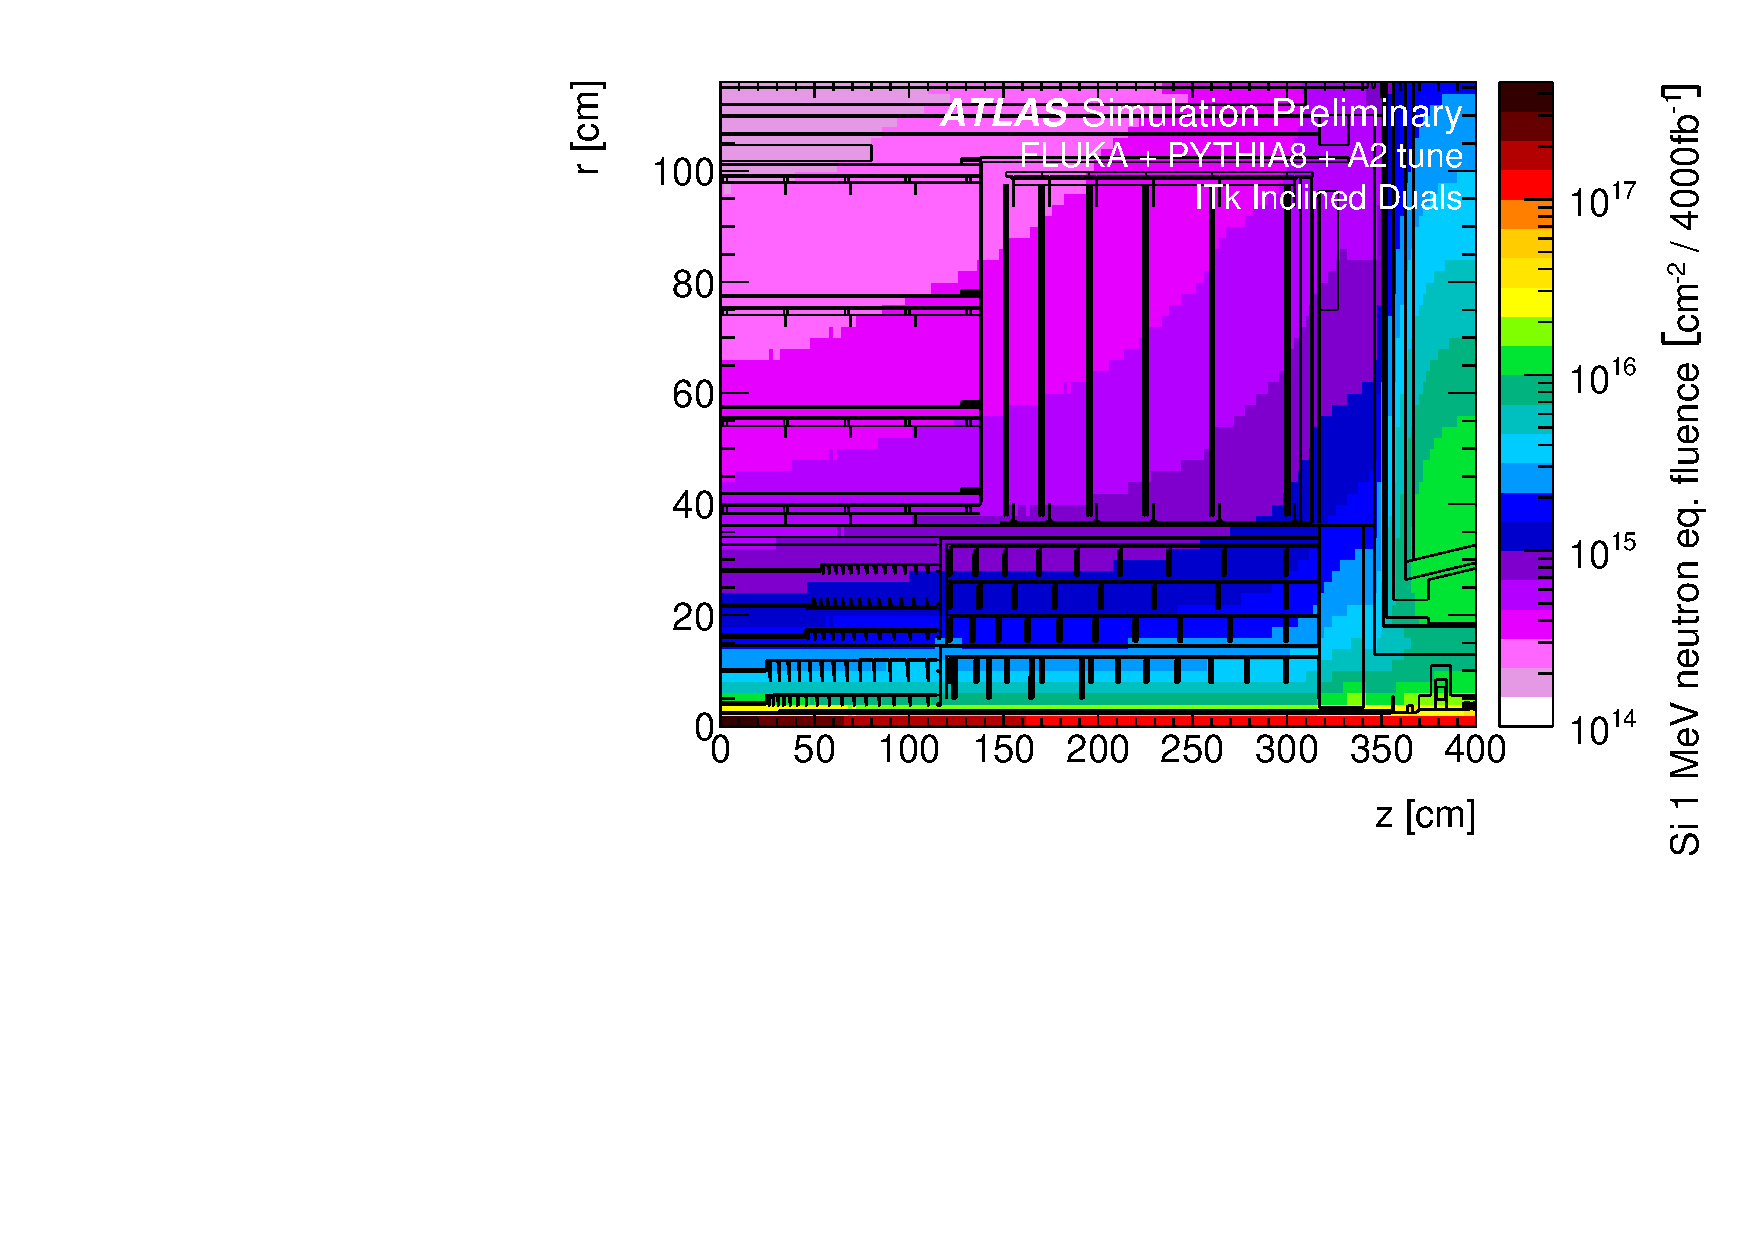
\includegraphics[width=0.48\linewidth]{figures/fluence.pdf}\quad
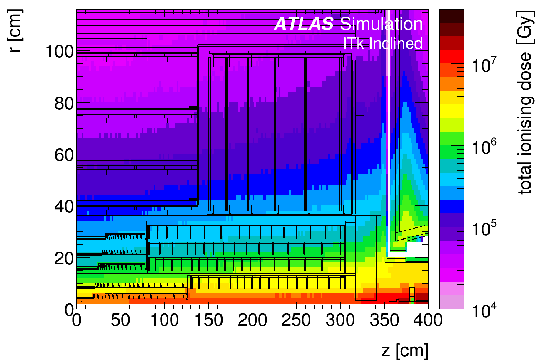
\includegraphics[width=0.48\linewidth]{figures/TID.pdf}
\caption{ATLAS ITk radiation environment. 1~MeV neutron equivalent fluence (left) and total ionizing dose (right). Both plots are for an integrated luminosity of 4000~fb$^{-1}$ \cite{Collaboration:2017mtb}.}
\label{fig:radiation}
\end{figure}


